\documentclass[a4paper, 12pt]{article}
%
%%%%%%%%%%%%%%%%%%%%%%%%%%%%%%%%%%%%%%%%%%%%%%%%%%%%%%%%%%%%%%%%%%%%%%
%
\PassOptionsToPackage{hyphens}{url}\usepackage[pdftex,
            bookmarksopen=true,
            colorlinks=true,
            linkcolor=blue,
            filecolor=blue,
            urlcolor=blue,
            citecolor=blue]{hyperref}
\hypersetup{%
  pdftitle = {User Guide-parMupSiF },
  pdfauthor = {Wendi Liu},
  pdfpagemode = UseOutlines
}
\usepackage{amsmath,amsfonts}
\usepackage{times}
\usepackage{graphicx}
\usepackage[usenames, dvipsnames]{color}
% \usepackage[plainpages=false,pdfpagelabels]{hyperref}
\usepackage[numbers]{natbib}
\usepackage{listings}
\usepackage{siunitx}
\usepackage{tikz}
\usepackage{hyperref}
\usepackage{dirtree}
\usetikzlibrary{trees}
%  \usepackage[top=length, bottom=length, left=length, right=length]{geometry} 
%%%%%%%%%%%%%%%%%%%%%%%%%%%%%%%%%%%%%%%%%%%%%%%%%%%%%%%%%%%%%%%%%%%%%%%%%
%% PAGE SET-UP
\topmargin30mm
\oddsidemargin30mm
\evensidemargin30mm
\textwidth150mm
\hoffset-26mm
\textheight236mm
\voffset-38mm
%% HEADER
%%%%%%%%%%%%%%%%%%%%%%%%%%%%%%%%%%%%%%%%%%%%%%%%%%%%%%%%%%%%%%%%%%%%%%%%%
\pagestyle{myheadings} 
\markboth{{\rm\small User Guide-parMupSiF}}
         {{\rm\small User Guide-parMupSiF}}
%%%%%%%%%%%%%%%%%%%%%%%%%%%%%%%%%%%%%%%%%%%%%%%%%%%%%%%%%%%%%%%%%%%%%%%%%       
% Sets for listings package
\definecolor{Mygreen}{rgb}{0,0.74,0}
\definecolor{turquoise}{cmyk}{0.49,0,0,0.29}
\definecolor{darkgray}{rgb}{0.95,0.95,0.95}
\definecolor{purple}{cmyk}{0.45,0.86,0,0}
\definecolor{lightred}{cmyk}{0.0,0.361,0.325,0}
\definecolor{lightgreen}{cmyk}{0.2,0.0,0.510,0}
\definecolor{CadetBlue}{cmyk}{0.4063,0.125,0.0,3725}
% Sets for listings package

\lstloadlanguages{C++,bash,csh}
\lstset{basicstyle=\small\ttfamily,frameround=ffff,language=[ISO]C++}
\lstset{backgroundcolor=\color{darkgray}}
\lstset{keywordstyle=\color{purple}\bfseries\emph}
\lstset{commentstyle=\color{blue}\itshape}
%%%%%%%%%%%%%%%%%%%%%%%%%%%%%%%%%%%%%%%%%%%%%%%%%%%%%%%%%%%%%%%%%%%%%%%%%
\newcommand{\dir}[1]{{\textbf{\color{blue}\texttt{#1}}}}
\newcommand{\exe}[1]{{\color{Mygreen}\texttt{#1}}}
\newcommand{\sub}[1]{{\color{purple}\texttt{#1}}}
\newcommand{\fort}[1]{{\color{turquoise}\texttt{#1}}}
%\newcommand{\file}[1]{{\begin{verbatin}{#1}\end{verbatin}}}
%%%%%%%%%%%%%%%%%%%%%%%%%%%%%%%%%%%%%%%%%%%%%%%%%%%%%%%%%%%%%%%%%%%%%%%%%  
%%%%%%%%%%%%%%%%%%%%%%%%%%%%%%%%%%%%%%%%%%%%%%%%%%%%%%%%%%%%%%%%%%%%%%%%%  

%\\begin{lstlisting}[frame=trBL,,escapechar=|]
%\[bash:$] code_saturne
%\Usage: /home/XXXXXX/SOFTWARE/SATURNE/5.0.8/code_saturne-5.0.8/\
%\arch/Linux/bin/code_saturne <topic>
%\
%\Topics:
%\help
%\studymanager
%\smgr
%\bdiff
%\bdump
%\compile
%\config
%\create
%\gui
%\studymanagergui
%\smgrgui
%\trackcvg
%\info
%\run
%\salome
%\submit
%\
%\Options:
%\-h, --help  show this help message and exit
%\\end{lstlisting}

\begin{document}
\title{User Guide -- Partitioned Multi-physical Simulation Framework }
\date{13/05/2020}
\maketitle
%
\begin{picture}(0,0)(50,-200)
\put(0,0){
\includegraphics[width=0.5\textwidth]{PICS/UKRI_STF_Council-Logo_Horiz-RGB.png}}    
\end{picture}
%%%%%%%%%%%%%%%%%%%%%%%%%%%%%%%%%%%%%%%%%%%%%%%%%%%%%%%%%%%%%%%%%%%%%%
%%%%%%%%%%%%%%%%%%%%%%%%%%%%%%%%%%%%%%%%%%%%%%%%%%%%%%%%%%%%%%%%%%%%%%

\section{Overview}

Partitioned Multi-physical Simulation Framework is developed based on the MUI library and offers a platform where users can carry out multi-physical (mainly fluid-structure interaction) studies with High Performance Computers developed and maintained by the fluid-structure interaction (FSI) team of SCD-STFC. 
The framework uses partitioned approach to couple two or more physical domains together for a multi-physical simulation. It takes several advantages of the MUI library that:
\begin{itemize}
	\item Flexible of select solvers for each physical domain;
	\item Flexible of extend the number of physical domains;
	\item Good scalability on communications among physical domains for large simulations.
\end{itemize}

Currently, the framework has implemented the coupling between Fluid solver and Structure for fully coupled FSI simulations:

\dirtree{%
	.1 Fluid-Structure Interactions.
	.2 Fluid Solver.
	.3 OpenFOAM\_V6.
	.2 Structure Solver.
	.3 FEniCS\_V2019.1.0.
	.2 Communicator.
	.3 MUI-1.0.
}


Figure \ref{fig:FSI_flow_chart} shows the flow chart of the present framework. The left hand side is the CFD solver for the fluid domain and the right hand side is the CSM solver for the structure domain. In the time step of $t=t+\delta t$ and sub-iteration $iter + 1$, the fluid domain solved the flow field and push the fluid forces at each cell of the fluid structure interface to the structural domain through the MUI library. The displacements at each cell of the interface were determined by the MUI coupling utility based on the fetched value from the structural domain. The calculated displacements of each cell at the interface were then applied to the fluid domain as a Dirichlet boundary condition. While the structural domain fetch fluid forces and applied as a Neumann boundary condition of the structure. It further calculated the deformation of the structure and push to the fluid solver. The stress of the structure will then be updated. Both fluid and structure domains were move to the next sub-iteration after the completion of the above actions. Several sub-iterations were needed within each time step until a convergence is reached, i.e. the $R_k$ is smaller enough that below the cretiria.

\begin{figure}
	\centering
	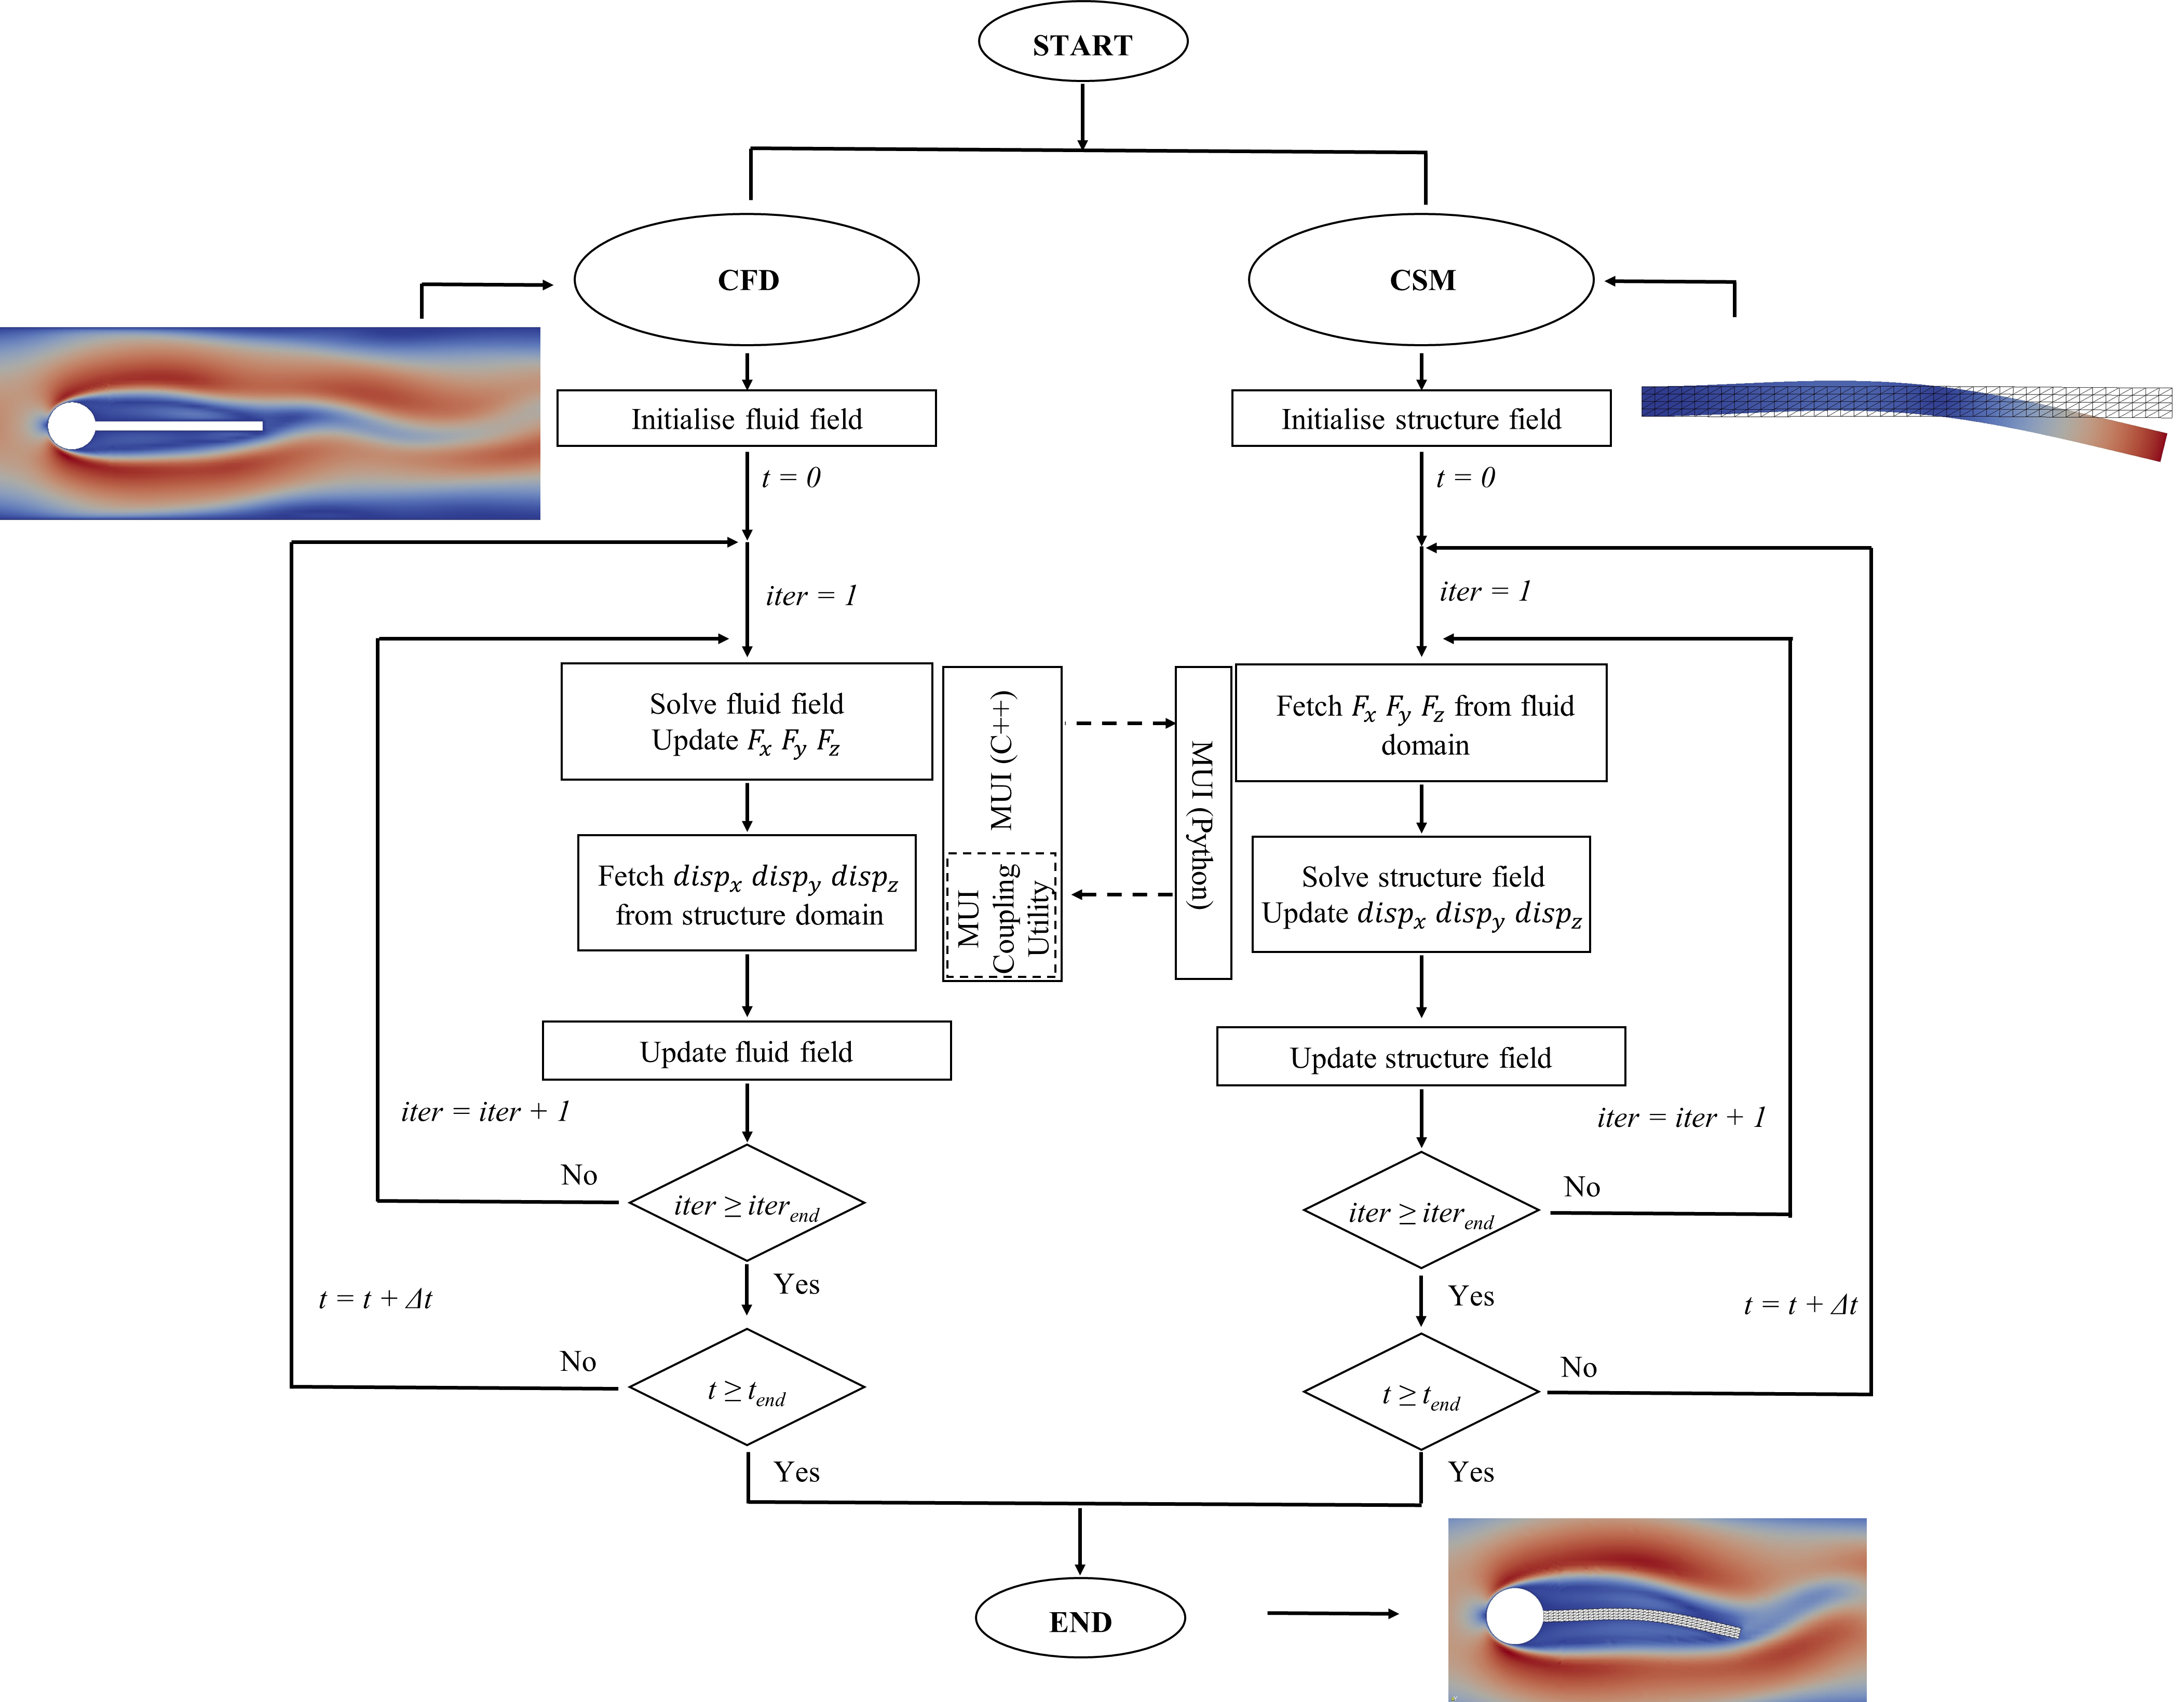
\includegraphics[width=1\columnwidth]{PICS/FSI_flow_chart.png}
	\caption{Flow chart of the simulation framework.}\label{fig:FSI_flow_chart}
\end{figure}

Apart from the loose coupling, the present framework also implemented both the Fixed Relaxation and the Aitken's $\delta^2$ methods with FSI sub-iterations implemented in both CFD and CSM solvers, as shown in Figure \ref{fig:FSI_flow_chart}. The Radial Based Function (RBF) that has been implemented in the MUI library was used to ensure the forces at the interface are conserved between the two domains. 

This framework is under active development to involve more solvers as well as more physical domains.
Such infrastructure will make it possible to simulate large multi-physical problems and simulate complicated multi-physical cases.

\section{Download}

The core code of the Partitioned Multi-physical Simulation Framework can be obtained from the GitLab:

\url{http://hcp004.hartree.stfc.ac.uk/wendi\_liu/FSI\_Simulation\_Framework.git}

\section{Installation}
Please follow the below steps to install the Framework:
\subsection{Step 1: Download and install FEniCS V2019.1.0}

\begin{itemize}
	\item Install pre-required modules:
	\begin{itemize}
		\item CMake V3.10+
		\item OpenMPI V2.1+
		\item Python V3.6+
		\item Eigen V3.3+		
		\item PETSc V3.7+
		\item Boost V1.68+
		\item Pybind11 V2.2+			
	\end{itemize}	
	\item Follow the instructions in \url{https://fenicsproject.org/download/} to download and install FEniCS\_V2019.1.0.

\end{itemize}

\subsection{Step 2: Download MUI library and install the MUI Python wrapper}

\begin{itemize}
	\item Download MUI V1.0 from \url{https://github.com/MxUI/MUI/archive/1.0.tar.gz}.
	\item Install pre-required modules:
	\begin{itemize}
		\item CMake V3.10+
		\item MPI4py V3.0+
		\item Python V3.6+
		\item OpenMPI V3.1.0
		\item numpy V1.13+
		\item Eigen V3.3+		
		\item Petsc V3.7+
		\item Pybind11 V2.2+			
	\end{itemize}
	\item source the FEniCS environment.
	\item Follow the instructions of README.md in the \dir{MUI/wrappers/Python} to install the Python wrapper of the MUI library.	
\end{itemize}

\subsection{Step 3: Download the Framework}

\begin{itemize}
	\item Download the Framework from \url{http://hcp004.hartree.stfc.ac.uk/wendi\_liu/FSI\_Simulation\_Framework.git}
\end{itemize}

\subsection{Step 4: and Download and install OpenFOAM V6}
	
	\begin{itemize}
		\item Clone a copy of the main OpenFOAM-6 repository (https://github.com/OpenFOAM/OpenFOAM-6) and associated ThirdParty-6 repository (https://github.com/OpenFOAM/ThirdParty-6).
		\item Extract the patch archive files from \dir{parMupSiF/src/MUI\_Utility/MUIpatchArchive-OpenFOAM\_6} into the base folder where cloned the two repositories
		\item Execute the script 
\begin{lstlisting}[frame=trBL,,escapechar=|] 
./patch\_OF6-MUI 
\end{lstlisting}
		\item Create an alias in the .bashrc file to "sourcing" OpenFOAM. i.e. edit \verb|.bashrc| in the home directory and add 
\begin{lstlisting}[frame=trBL,,escapechar=|] 
alias of6='source [path to where cloned the OpenFOAM-6 directory]
/etc/bashrc; export WM\_NCOMPPROCS=8' 
\end{lstlisting}
		\item Re-source \verb|.bashrc| script using 
\begin{lstlisting}[frame=trBL,,escapechar=|] 
source .bashrc 
\end{lstlisting}
		\item Trigger the alias by typing  
\begin{lstlisting}[frame=trBL,,escapechar=|] 
of6 
\end{lstlisting} 
		there should see no errors
		\item In the ThirdParty-6 folder, place a full copy of MUI library into the new folder \verb|MUI| (these can be sym links but make sure they are not relative paths as a script takes a copy of these files, whenever update MUI the old platform files need to clean and re-run \verb|Allwmake| to update the copy that gets used by the OpenFOAM applications).
		\item Build the ThirdParty libraries with \verb|Allwmake|
		\item Build OpenFOAM-6 itself using \verb|Allwmake| in the base of the repository folder (as usual)
		\item There is a sample coupled case using \texttt{laplacianFoam} in \\ \dir{tutorials/basic/laplacianFoam}
	\end{itemize}
	
\subsection{Step 5:Install the OpenFOAM solver \texttt{pimpleFSIFoam}}
	\begin{itemize}
		\item Go to \dir{parMupSiF/src/CFD/OpenFOAM/V6/parmupsifLibs}.
		\item run 
\begin{lstlisting}[frame=trBL,,escapechar=|] 
./Allwmake
\end{lstlisting} 
		to compile the solver \texttt{pimpleFSIFoam} and boundary conditions \texttt{parmupsifBC}
	\end{itemize}

\section{Folder Structure}

\dirtree{%
	.1 parMupSiF.
	.2 config.
	.3 parmupsif\_gcc.conf \textit{[Configure files for Scafell Pike]}.
	.2 demo.
	.3 couplingLibDemo \textit{[Demo case for MUI coupling utility]}.
	.3 cylinderFlap \textit{[Demo case on 2D FSI simulations]}.
	.3 FSIBeam \textit{[Demo case on 3D FSI simulations]}.
	.3 Structure\_validation \textit{[Demo case on the in-house FEniCS solver]}.
	.2 docs.
	.3 ToDo\_List.
	.3 UserGuide.
	.2 src.
	.3 CFD.
	.4 OpenFOAM.
	.5 V6.
	.6 parmupsifLibs \textit{[the solver \texttt{pimpleFSIFoam} and boundary conditions \texttt{parmupsifBC}]}.
	.3 CSM.
	.4 FEniCS.
	.5 V2019.1.0.
	.6 structureFSISolver \textit{[the in-house FEniCS structure solver]}.
	.3 MUI\_Utility.
	.4 couplingLab \textit{[the MUI coupling utility]}.
	.4 MUIpatchArchive-MUI\_dev \textit{[the patch archive files to modify MUI library on its RBF sampler]}.
	.4 MUIpatchArchive-OpenFOAM\_6 \textit{[the patch archive files to merge MUI library into OpenFOAM V6]}.
	.2 thirdparty.
	.3 eigen \textit{[third party libraries (i.e. Eigen)]}.
	.1 README.md.
}

\section{Demo Cases}

The Framework provided several demo cases. Taking the demo case on 3D FSI simulations \verb|FSIBeam| as an example, the folder structure for a simulation case is as follows:

\dirtree{%
	.1 FSIBeam.
	.2 caseSetup \textit{[contains the original settings of the simulation for both fluid and structure solvers]}.
	.3 fluidDomain \textit{[contains the original settings of the simulation for the fluid solver]}.
	.3 structureDomain \textit{[contains the original settings of the simulation for the structure solver]}.
	.2 runCtrl \textit{[contains the utilities for the simulation]}.
	.2 Allclean \textit{[clean all the running results]}.
	.2 Allrun \textit{[run the simulation]}.
	.2 FlexBeam1e6.sh \textit{[Job script for Scafell Pike]}.
}

After running, another folder will be generated to contain the simulation results:
\dirtree{%
	.1 FSIBeam.
	.2 caseSetup.
	.2 runCtrl.
	.2 runData \textit{[Results folder]}.
	.3 fluidDomain \textit{[contains the results from the fluid solver]}.
	.3 logFiles \textit{[contains the log files for the entire simulation]}.
	.3 structureDomain \textit{[contains the results from the structure solver]}.
	.4 dataInput \textit{[contains the mesh for the structure solver]}.
	.4 structureFSISetup \textit{[contains the set-up for the structure solver]}.
	.4 structureResults \textit{[contains the results from the structure solver]}.
	.4 structureDomainRun.py \textit{[high-level script for the structure solver]}.
	.2 Allclean.
	.2 Allrun.
	.2 FlexBeam1e6.sh.
}


\end{document}
